\documentclass[7pt]{article}
\twocolumn
\usepackage[utf8]{inputenc}
\usepackage{graphicx}
\usepackage{subcaption}
\usepackage{caption}
\usepackage{siunitx}
\usepackage{hyperref}
\graphicspath{{./images/}}
\usepackage{amsmath}

\usepackage{natbib}
\bibliographystyle{abbrv}
\usepackage[superscript,biblabel]{cite}

\usepackage[a4paper, total={183mm, 247mm}]{geometry}
\usepackage[switch]{lineno}
\linenumbers

\newcommand*{\ts}{{\tau^{*}}}
\newcommand*{\diff}{\mathop{}\!\mathrm{d}}
\newcommand{\ps}{\si{\pico\second}}
\newcommand{\ns}{\si{\nano\second}}
\newcommand{\fs}{\si{\femto\second}}
\newcommand{\ips}{\si{\per\pico\second}}
\newcommand{\us}{\si{\micro\second}} 
\newcommand{\iA}{\si{\per\angstrom}}
\newcommand{\K}{\si{\kelvin}} 
\newcommand{\amu}{\si{\amu}} 
\newcommand{\uzeta}{\si{\pico\second\per\angstrom\squared}}
\newcommand{\THz}{\si{\tera\hertz}}

\usepackage{sectsty}
\sectionfont{\small}

\title{Reductionism, surface dynamics and the Kramers problem}

\author{Jeremy Wilkinson}
\date{September 2021}

\begin{document}

\maketitle

The development of experimental methods such as helium spin-echo microscopy\cite{FouquetHSEM, JardineHSEM} and inelastic neutron scattering\cite{Wright1983} marked a revolution in the ability to observe the diffusion of adatoms over a substrate. While the observables in a surface scattering experiment contain a certain statistical description of adatom motion\cite{vanHowe}, the microscopic trajectories of adatoms are not directly observable. The nature of microscopic adatom motion from which macroscopic observable quantities emerge therefore remains open to conjecture. Little can be known about the exact state of a substrate and its interactions with an adsorbate, yet physical properties emerge which can be reliably defined and measured with complete ignorance to the vast majority of information in the system. The questions therefore arise, \emph{what are the relevant observable quantities in a system} and \emph{what is the minimum amount of information needed to explain these observables}. The answers to these questions influence what parameters are used to classify systems and guide the exploration of new materials. Through theoretical and computational study, we expand upon these questions in the context of low temperature surface diffusion, with conclusions that carry over to the many activated processes modeled by the Kramer's problem. 


\section*{Surface diffusion}

\begin{figure}
	\centering
	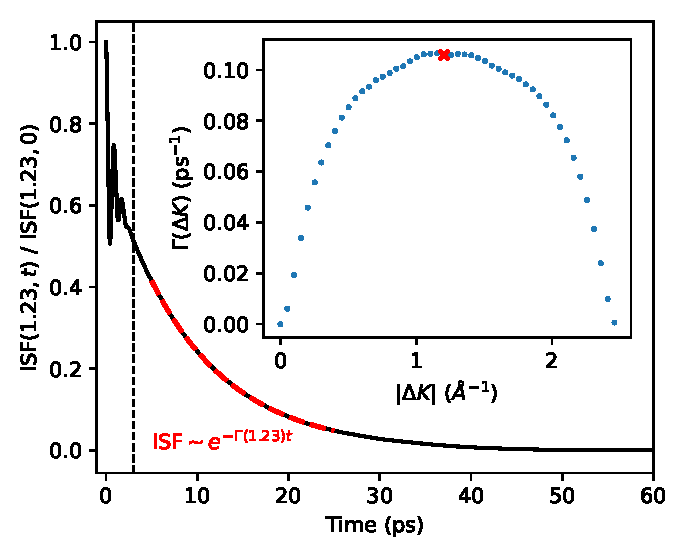
\includegraphics[width=1.0\columnwidth]{isf_dk}
	\caption{The main axes show a typical ISF over time for a fixed momentum transfer. The decay rate, $\Gamma$, of the ISF's exponential tail is proportional to the hopping rate of the adatom. By calculating $\Gamma$ over a range of momentum transfers a jump distribution plot may be constructed, as shown in the inset axes.} 
	\label{fig:isf_dk}
\end{figure}

At low temperatures, surface diffusion is predominantly a classical activated diffusion process\cite{} wherein adatoms are bound to local minima in the substrate potential, referred to as adsorption sites. As an adatom oscillates about its local adsorption site it is able to slowly exchange energy with the substrate through interactions with surface phonons. On occasion, the adatom will find itself with enough energy to overcome the trapping potential and is able to hop to an adjacent site, or further. The hopping rate and distribution of jump lengths set the rate of macroscopic diffusion over the surface and are strongly influenced by the shape of the trapping well, in particular the activation energy, as well as the rate at which the adatom exchanges energy with the substrate.

The rate of hopping, $\gamma$, is usually observed to obey an Arrhenius law, of the form $\gamma = A\exp\left(-E_a/k_BT\right)$, with an associated activation energy, $E_a$ and a pre-exponential factor $A$. The exponential Boltzmann factor serves as a quantifier of the number of particles with sufficient energy to clear the potential barrier at equilibrium while the pre-exponential factor contains all other dynamical information and is in principal a complicated functional of the potential well, the energy exchange rate and the substrate-adatom interactions. 

While it is relatively simple to extract an activation energy directly from experimental data\cite{Diamant,Alexandrowicz2006}, it is not possible to disentangle the energy exchange rate of the system from other effects without making further assumptions. The most common approach is to assume that the force on the particle may be treated as a random variable obeying the Markovian Langevin equation,
\begin{equation}
\begin{gathered}
	m\ddot{\vec{r}}=-m\eta\dot{\vec{r}}-\nabla U(\vec{r})+\vec{f}(t) \\ 
	\text{ where } \left<f(t_1)f(t_2)\right>=2k_BTm\eta\delta(t_1-t_2),
\end{gathered}
	\label{eq:langevin}
\end{equation}
and to fit the experimental data with simulated solutions to the Langevin equation. The resulting best fit friction parameter, $\eta$, parameterizes the strength of the random force $\vec{f}$ and may be used as a quantifier of the rate of energy transfer with the substrate. Theoretical results for the escape rate of a Markovian Langevin particle from a one dimensional potential well indicate that one expects a pre-exponential factor which is proportional to the friction constant $\eta$ in the low friction regime\cite{Kramers, Zwanzig}. 

Other than their attractive simplicity, the use of a friction term strictly linear in the instantaneous velocity and a random force completely uncorrelated in time are difficult to justify a priori. Attempts by the authors to directly observe the force distribution on an adatom in a full 3D molecular dynamics simulations have yet to demonstrate Langevin type statistics, suggesting that the statistics involved are more sophisticated. Furthermore, in the Fourier domain, uncorrelated noise corresponds to a uniform power spectrum $\left<\tilde{f}(\omega_1)\tilde{f}(\omega_2)\right>=4\pi k_BTm\eta\delta(\omega_1+\omega_2)$. However, the source of noise in a surface dynamics system, the substrate phonons, have a well defined maximum vibrational cutoff frequency, on the order of a few terahertz, and therefore the force they exert must be correlated in time\cite{Sinha}. The Markovian Langevin approach has nevertheless been used to successfully fit the long-time observables in both physical systems\cite{} and three dimensional simulations\cite{Diamant}, for reasons which will become clear through the results presented. 

The observable quantity in a surface scattering experiment is the intermediate scattering function,
$$
\mathrm{ISF}(\Delta{\vec{K}}, t) = \left<\exp\left(i\Delta{\vec{K}}\cdot\vec{r(t)}\right)\right>.
$$
The ISF is typically quoted for a single momentum transfer, $\Delta{K}$, over a range of time, as shown in the main axes of Fig. \ref{fig:isf_dk}. For the purposes of extracting the long-time average rate of diffusion over the surface, the exponential decay rate of the ISF at long times, $\Gamma(\Delta{\vec{K}})$, is the quantity of interest and is proportional to the adatom hopping rate\cite{Chudley}. By varying the magnitude of $\Delta{K}$ in a particular direction, one may calculate the jump distribution plot as shown in the inset of Fig. \ref{fig:isf_dk}. When an adatom escapes from a well, it may hop more than one site before it settles down again. The shape of the jump distribution is set by the relative probability of the number of sites an adatom travels before settling down again \cite{Chudley}. Therefore one may compare the hopping rate and hop length distributions of two systems through the amplitude and shape of their jump distributions.

The consequences of ignoring the true microscopic statistics of a system were previously unknown but are explored in this work through the comparison of four models of microscopic motion which manifest fundamentally different friction and noise forces. The differences in macroscopic properties are quantified and are found to be largely independent of the choice of the microscopic motion provided the equilibrium statistics and a single energy exchange rate parameter are kept fixed. 

\section*{Computational Models}

In addition to the aforementioned Markovian Langevin equation, we present three models for the microscopic motion of adatoms. The first is a generalized form of the Langevin equation which incorporates correlations in the noise force through convolution with a memory Kernel, $K(t)$. The preservation of Boltzmann statistics requires that both the friction force and the noise force be modified, resulting in the generalized Langevin equation\cite{Kubo},
\begin{equation}
	m\ddot{\vec{r}}+m\eta\int_0^t\diff{t'}K(t-t')\dot{\vec{r}}(t')+\nabla U(\vec{r})=\int_0^t\diff{t'}\vec{f}(t')K(t-t').
	\label{eq:gle}
\end{equation}
An exponential memory kernel, $K(t)=\frac{1}{\tau}\exp\left(-\frac{t}{\tau}\right)$, parameterized by a noise correlation time $\tau$ was used to generate a noise power spectrum given by $\tilde{K}(\omega)=\frac{1}{1+\omega^2\tau^2}$ and a bandwidth of $\omega_\text{cutoff}=\frac{1}{\tau}$. In the limiting case of $\tau=0$, the white noise of the Markovian Langevin equation is recovered. 

In his seminal work on Brownian motion, Kramers points out, that the laws of friction which result in a Boltzmannian phase space distribution at equilibrium are not unique and that the linear friction in Eq. \ref{eq:langevin} is nothing more than the simplest possible case\cite{Kramers}. The consequences of using an alternative friction law are explored through the second model, a Markovian Langevin equation with a cubic friction force parameterized through $\zeta$,
$$
m\ddot{\vec{x}} + m\zeta\dot{x}^2\dot{\vec{x}} + m \nabla U(x) = \vec{f}(t),
$$
along with a modified fluctuation-dissipation theorem\cite{Kramers},
$$\left<f(t_1)f(t_2)\right>=\left(4\zeta\left(k_BT\right)^2 + 2 m \zeta \left(k_BT\right)\dot{x}^2(t_1)\right)\delta\left(t_1-t_2\right).$$

The final model presented is a full 3D molecular dynamics simulation of sodium on copper(001) which tracks the harmonic interactions and motion of each copper atom in an $8\times8\times8$ substrate as well as the interactions with a sodium adatom via a Morse potential. The simulation parameters determined by Ellis and Toennies\cite{Ellis} were optimized to fit the binding energy, activation energy and vibrational frequency of Na on Cu(001). This model reproduces the phonon dispersion relation of a real copper crystal\cite{Sinha} and therefore provides a realistic model of three dimensional phonon-adatom interactions.

The two dimensional free energy surface parallel to the substrate was extracted from the 3D simulation through the density function of a microcanonical ensemble of trajectories and the definition,
$$U(\vec{x}) = -kT\log\left(\left<\delta^{(2)}(\vec{r}_{\parallel}(t) - \vec{x})\right>\right).$$
This potential, shown in Fig. \ref{fig:pot_surface}, was used as the background potential of the Langevin type simulations. Each model therefore attains the same two dimensional equilibrium phase space distribution, albeit through different microscopic statistics. 

\begin{figure}
	\centering
	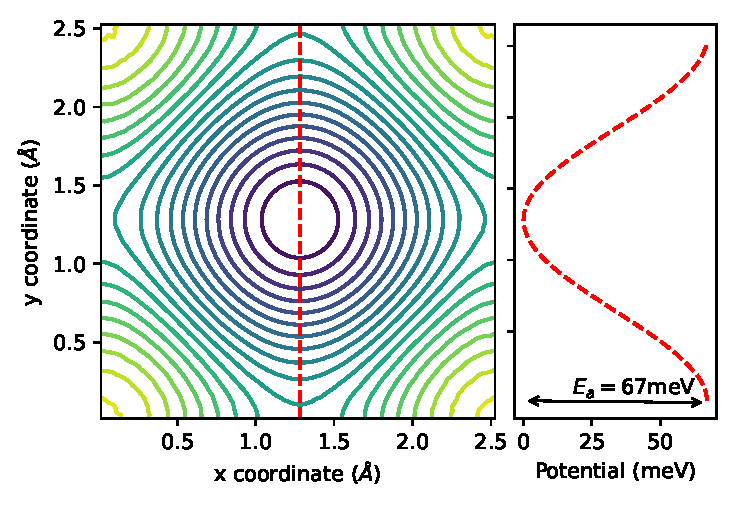
\includegraphics[width=1.0\columnwidth]{pot_surface}
	\caption{The potential energy surface extracted from the sodium on copper(001) 3D molecular dynamics simulation with a superimposed trajectory typical for a low friction activated diffusion process. The red dashed line in the right panel shows a cross section of the potential through an adsorption site and two bridge sites as annotated in the panel on the left. All ISFs presented in this paper are quoted with the a momentum transfer pointing from the adsorption site through one of the equivalent bridge sites}
	\label{fig:pot_surface}
\end{figure}

\section*{Energy exchange rates}

\begin{figure}
	\centering
	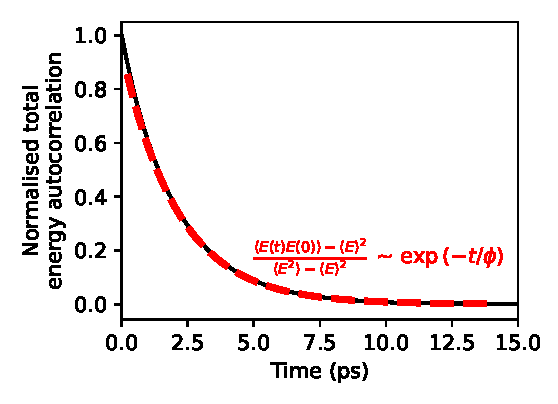
\includegraphics[width=1.0\columnwidth]{e_auto}
	\caption{A typical total energy auto-correlation function notably absent of any oscillations which are generally present in a kinetic energy correlation function. Since the decay is generally not a pure exponential, the total energy correlation time $\phi$ is defined as the interval over which the normalized auto-correlation function drops to $1/e$.}
	\label{fig:e_auto}
\end{figure}

\begin{figure*}
	\centering
	\includegraphics[width=0.8\textwidth]{energy_exchange_rates}
	\caption{The top left panel shows the variation of the energy exchange rate as a function of the friction parameter, $\eta$, and noise correlation time $\tau$ in the linear friction Langevin models. The suppression factor, $I$, of the non-Markovian Langevin model is shown in the top right panel and the bottom left panel shows the energy exchange rate as a function of the cubic friction coupling constant $\zeta$. I am considering removing the bottom right panel.}
	\label{fig:energy_exchange_rates}
\end{figure*}

While the fraction of time spent above the activation energy is set by Boltzmann statistics, the number of times this energy level is attained independently per unit time is set by the energy exchange rate. For this reason, we define the energy exchange rate as the inverse of the correlation time, $\phi$, of the \emph{total energy} auto-correlation function, $$\frac{\left<E(t)E(0)\right> - \left<E\right>^2}{\left<E^2\right> - \left<E\right>^2},$$ as shown in Fig. \ref{fig:e_auto}. Each simulation was run for a total of $2\us$ across a range of parameters and the observed energy exchange rates are summarized in Fig. \ref{fig:energy_exchange_rates}. 
 
The introduction of noise correlations was found to suppresses the energy exchange rate with the substrate, as shown in the top panel of Fig. \ref{fig:energy_exchange_rates}. For the sake of comparison, the red line shows the energy exchange rate of a particle with Markovian Langevin statistics in a harmonic well, $\phi^{-1}=\eta$. For short correlation times, we find the energy exchange rate is close to $\eta$, but even for $\tau=0$, there are small differences due to anharmonicities in the background potential. As the noise correlation time approaches $0.4\ps$, the energy exchange rate is seen to fall by close to a factor of four, demonstrating that the narrowing of the noise power spectrum can have a large effect on the energy exchange rate. Regardless of the noise correlation time, the exchange rate was found to remain linear in $\eta$ suggesting that $\eta$ acts as an overall interaction strength parameter while $\tau$ controls the coupling strength to individual modes, suppressing interactions with high frequency modes. 

This suggests the introduction of a dimensionless, $\eta$ independent, suppression factor, $I = \frac{\phi^{-1}}{\eta}$, which quantifies the suppression of energy exchange as a function of $\tau$. The suppression factor for the non-Markovian simulation is shown in the top right panel of Fig. \ref{fig:energy_exchange_rates} alongside the analytic suppression factor of an equivalent system in a harmonic well of natural frequency $\omega_0$. The toy model is solved in the supplemental information and is found to admit a similar $\eta$ independent suppression factor in the low friction limit. Within this simplified model, the suppression effect can be understood by considering the expected energy change of the adatom when subjected to a single noise impulse which decays in time as $K(t)$. Without loss of generality, we suppose the impulse begins when the particle is passing through the potential minimum of an oscillation, and is oriented in the direction of motion. If $K(t)$ decays quickly compared to the oscillation period, then $K(t)$ is imparted entirely in the direction of motion, and the adatom quickly settles into a new, higher energy level. If $K(t)$ decays at a rate comparable to the oscillation period of the well then the noise force acts against the direction of motion as it passes through the minimum again in the opposite direction and removes some of the energy it imparted, effectively interfering with itself. The new energy level attained is therefore not as high as in the former case and we therefore expect a lower change in the total energy per impulse. A similar argument can be made for the correlated friction force removing less energy per oscillation. This interpretation is reflected in the mathematical form of the low friction approximation of the harmonic well's suppression factor as an oscillating integral over $K(t)$,
$$
$$
\begin{equation}
	I(\tau, \omega_0) = \frac{1}{1+\left(\omega_0\tau\right)^2} = \int_0^{\infty}\diff{t}K(t)\cos{\omega_0t},
	\label{eq:suppression_factor}
\end{equation}
which coincides with the power spectrum of the memory kernel. We therefore find that the energy exchange rate of a particle oscillating with angular frequency $\omega_0$ is suppressed to the same degree as the amplitude of the noise power spectrum around $\omega_0$. 

The energy exchange rate of the cubic friction model, shown in the bottom left panel of Fig. \ref{fig:energy_exchange_rates}, was found to be linear in $\zeta$, with energy exchange rates comparable to the linear friction models when $\zeta$ is on the order of $10^{-5}\uzeta$.

\section*{Hopping rates}

\begin{figure}
	\centering
	\includegraphics[width=1.0\columnwidth]{gamma_ttf}
	\caption{A scatter of the maximum ISF dephasing rate, $\Gamma_{\text{max}}$, against the energy exchange rate, $\phi^{-1}$, for each microscopic model demonstrates that the ISF dephasing rate is set by the energy exchange rate and the potential background with other microscopic details accounting for less than $3\%$ of the variance in the limit of low energy exchange rate.}
	\label{fig:gamma_ttf}
\end{figure}

\begin{figure}
	\centering
	\includegraphics[width=1.0\columnwidth]{jump_distribution}
	\caption{Each scatter shows the jump distribution of a particular microscopic model for three different energy exchange rates, $0.3$, $0.5$ and $0.7\ips$. A noise correlation time of $0.1\ps$ was used for the non-Markovian model in each instance.} 
	\label{fig:jump_distribution}
\end{figure}

As a measure of the total hopping rate, The peak of the jump distribution, $\Gamma_{\text{max}}$ (annotated in Fig. \ref{fig:isf_dk}), was calculated for each model. The small round points in Fig. \ref{fig:gamma_ttf}, show that the energy exchange rate of the non-Markovian Langevin equation is an excellent estimator for the total hopping rate of the system. The color of the markers demonstrates that for fixed $\eta$, the total hopping rate can vary by many multiples when the noise correlation time is adjusted. However when considered as a function of a fixed energy exchange rate, the hopping rate is found to vary by less than $3$\%, a portion of which may be attributed to statistical error. We therefore find that noise correlations do in fact have an effect on an adatom's hopping rate, however to first order, this effect only occurs through the the energy exchange rate and can therefore be compensated for through an adjustment of $\eta$.

The cubic model's hopping rate was found to vary linearly as a function of the coupling $\zeta$, however once again, if the energy exchange rate is tuned to match the exchange rate of the linear friction models, the hopping rate is found to lay within a few percent of the linear friction models.

The shape of the jump distribution of each model was compared by tuning the available parameters to run each model over a fixed set of energy exchange rates. The jump distributions for each model at the energy exchange rates $0.3$, $0.5$, and $0.7\ips$ are shown in Fig. \ref{fig:jump_distribution}. The jump distributions presented are normalized to peak at the same height within each energy transfer rate to allow for the comparison of the jump distribution shape. For a fixed energy exchange rate, the adatom jump distribution shapes were found to agree well across all models with only small differences in the overall shape. The peaks of the jump distributions at higher exchange rates are all observed to be narrower than those at lower exchange rates, indicating an increase in the probability of single hops to adjacent sites\cite{Diamant}. This is expected as higher energy exchange rates decrease the probability that a particle which has escaped its well finds another bridge site before attaining an independent energy level likely lower than the activation energy and being bound to an adjacent well.

Taken together, the hopping rate and jump distribution fully specify the long-time characteristics of activated diffusion systems. The results presented demonstrate that the microscopic details of adatom motion such as the noise bandwidth, or the exact form of friction force, can effect motion over long timescales, however, to first order only through the energy exchange rate. 

\section*{Discussion}

These conclusions validate the standard approach of classifying a given system through a single energy exchange rate parameter and a set of parameters which specify the details of the background potential. It is apparent that any effects attributable to the differences in microscopic statistics have been safely ignored until this point as they can be compensated for by adjusting the energy exchange rate through whichever parameters are available in the model of choice.

While an exponential memory kernel was used in these simulations for computational efficiency, the hard phonon cutoff in real systems is likely to induce oscillations in the memory kernel, akin to a sinc function. When the period of oscillations in the adsorption site match those of the memory kernel, the potential for resonance effects becomes apparent. The vibrational frequency of an adatom can be measured directly using helium spin-echo and the surface phonon spectrum can be measured using techniques such as Neutron scattering\cite{Sinha}. By exploring various substrate-adsorbate combinations, it may be possible to observe the harsh drop in the hopping pre-exponential factor predicted by Eq. \ref{eq:suppression_factor} in system for which the vibrational frequency exceeds the phonon cutoff frequency. However, multiple properties contribute to the pre-exponential factor and it therefore may be difficult to see the proposed trend in physical systems. 


\bibliography{bibliography}

\end{document} 
